%!TEX encoding = UTF-8 Unicode

\documentclass{article}


\usepackage{arxiv}
% \usepackage{graphicx}
% \usepackage[utf8]{inputenc} % allow utf-8 input
% \usepackage[T1]{fontenc}    % use 8-bit T1 fonts
% \usepackage{hyperref}       % hyperlinks
% \usepackage{url}            % simple URL typesetting
% \usepackage{booktabs}       % professional-quality tables
% \usepackage{amsfonts}       % blackboard math symbols
% \usepackage{nicefrac}       % compact symbols for 1/2, etc.
% \usepackage{microtype}      % microtypography
% \usepackage{lipsum}

%%% ============================DOCUMENT SET UP=========================
%	documentclass sets up the type of document
% \documentclass[a4paper,12pt]{article} % options font size, etc.
%	inputenc  sets up the input enconding
	\linespread{1.15}
%\usepackage[utf8]{inputenc} % utf8, etc.
%	fontenc	  necessary to encode special characters like ä, ö, ß usw.
\usepackage[T1]{fontenc}
%	babel			adds capabilites for working correctly with other languages
%\usepackage[german]{babel} % not necessary for english
%	hyphennat	some words are incorrectly hyphenated, for these in textmode,
						% a special command may be inserted e.g. \hyphenation{so-wieso}
\usepackage{hyphenat}
% Use specific fonts only works with xelatex or lulatex
% \usepackage{fontspec}
% %\defaultfontfeatures{Mapping=tex-text,Scale=MatchLowercase}
% 	\defaultfontfeatures{Mapping=tex-text}
% 	\setmainfont[BoldFont = timesbd.ttf,
% 							 ItalicFont = timesi.ttf,
% 							 BoldItalicFont = timesbi.ttf]{times.ttf}
% % Sans Font is normally used for headings. If it's set to times new roman, all is well
%  	\setsansfont[BoldFont = timesbd.ttf,
%  							 ItalicFont = timesi.ttf,
%  							 BoldItalicFont = timesbi.ttf]{times.ttf}

	%\setmainfont[BoldFont = arialbd.ttf,
	%						 ItalicFont = ariali.ttf,
	%						 BoldItalicFont = arialbi.ttf]{arial.ttf}

%%  ----------------------------TABLE OF CONTENTS-----------------------
%	tocbibind	Put the bibliography in the ToC
% if list of figures should be excluded add notlof for list of tables notlot
\usepackage[nottoc]{tocbibind}
% tocloft		Alter the style of the Table of Contents
						% needs to be before parskip, warning @startoc has changed can
						% then probably be ignored
\usepackage[titles]{tocloft} % option subfigure
	\renewcommand{\cftsecfont}{\rmfamily\mdseries\upshape}
	\renewcommand{\cftsecpagefont}{\rmfamily\mdseries\upshape} % No bold!

% create a list of hypotheses
\usepackage[hyperref]{ntheorem}
	\theoremstyle{plain}
	\theoremnumbering{arabic}
	\theoremindent 5mm
	\theoremseparator{:}
	\newtheorem{Hypothesis}{H}

\def\subsectionautorefname{Section}
\def\subsubsectionautorefname{Section}
\def\subsubsection
\def\paragraphautorefname{Section}
\newcommand*{\Appendixautorefname}{Appendix}
\def\figureautorefname{Figure}
\def\tableautorefname{Table}

%%  ----------------------------BIBLIOGRAPHY----------------------------
% natbib		flexible bibliography (works with citep and citet amon others
\usepackage[round, semicolon, authoryear]{natbib}
	\bibliographystyle{humannat} % sets the bibliographystlye

%%  ----------------------------GLOSSARY--------------------------------
%	glossaries package for using index, acronyms, glossary, symbols, etc.

\usepackage[nopostdot,nonumberlist,acronym,toc,nomain, nogroupskip]{glossaries}
\usepackage{glossary-superragged}
\setglossarystyle{superragged}
\renewcommand{\glsdescwidth}{.75\linewidth}
%%  ----------------------------APPENDIX--------------------------------
\usepackage[toc,page]{appendix}

%%% ============================PAGE SETUP==============================
% geometry	to change the page dimensions
\usepackage{geometry}
	\geometry{a4paper}
 	\geometry{margin=1in} % for example, change the margins to 2 inches all round
%	parskip		Activate to begin paragraphs with an empty line rather than an indent
\usepackage[parfill]{parskip}
% nowidow   does not allow widowed lines in the output document
\usepackage[all]{nowidow}
%	sectsty		changes the appearance of section titles
\usepackage{sectsty}
	\allsectionsfont{\sffamily\mdseries\upshape} % (See the fntguide.pdf for font help)

%	topfraction Legt den Anteil des Platzes am oberen Rand einer Seite fest, bis
% zu dem Gleitobjekte plaziert werden können.
\renewcommand{\topfraction}{.85}

\def\blankpage{%
      \clearpage%
      \thispagestyle{empty}%
      \addtocounter{page}{-1}%
      \null%
      \clearpage}
%%  ----------------------------HEADERS & FOOTERS-----------------------
%	fancyheadr This should be set AFTER setting up the page geometry
\usepackage{fancyhdr}
	\pagestyle{fancy} % options: empty , plain , fancy
	\renewcommand{\headrulewidth}{0pt} % customise the layout...
% footmisc	alter the style of footnotes
\usepackage[hang,flushmargin]{footmisc} % options hang and flushmargin set
                                        % remove the indent of footnotes


%%% ============================ENVIRONMENTS============================
%	float     let latex arrange figures and tables
\usepackage{float}
%	verbatim	adds environment for commenting out blocks of text & for better verbatim
	\usepackage{verbatim}

%%  ----------------------------TABLES & LISTS--------------------------
% tabularx  makes creating tables much easier
\usepackage{lscape}
\usepackage{tabularx}
\usepackage{multirow}
	% newcolumntype can be used to define colums which can later be used in tables
	\def\tabularxcolumn#1{m{#1}}
	\newcolumntype{M}{>{\hsize=.75\hsize\centering}X} % small & centered columns
	\newcolumntype{I}{>{\hsize=.75\hsize}X} % small & centered columns
	\newcolumntype{C}{>{\centering\arraybackslash}X}
	\newcolumntype{S}{>{\hsize=.5\hsize\centering}X} % small & centered columns
	\newcolumntype{L}{>{\hsize=1.25\hsize\centering\arraybackslash}X} % small & centered columns

% booktabs	for much better looking tables
\usepackage{booktabs}
% longtable supports footnotes in tabular environments
\usepackage{threeparttable}
% paralist	very flexible & customisable lists (eg. enumerate/itemize, etc.)
\usepackage{paralist}
% grids
\usepackage{tikz}
%%  ----------------------------FIGURES---------------------------------
%	graphicx 	support the \includegraphics command and options
\usepackage{graphicx}
%	subcaption	add captions to each subfigure in a figure environment
\usepackage{subcaption} % not possible to use with subfig
\usepackage[font=small]{caption}
\captionsetup[table]{skip=.25\baselineskip, singlelinecheck = false, justification=justified}

%%	----------------------------MATH & CHEMISTRY------------------------
%	amsmath		numbered euqations which are in equation environments
\usepackage{amsmath}
\usepackage{mathtools}
%	array		for better arrays (eg matrices) in maths
\usepackage{array}
%	enable chemistry in mathmode. Formatting is not as nice.
% \newcommand*\chem[1]{\ensuremath{\mathrm{#1}}}
% advanced chemistry mode
\usepackage[version=4]{mhchem}

%%	----------------------------SYMBOLS & FORMATTING--------------------
%	textgreek	in text greek letters, without activating mathmode
\usepackage{textgreek}
%	textcomp	adds symbols in textmode
\usepackage{textcomp}
%	amssymb		adds further symbols
\usepackage{amssymb}  % add further symbols
%	color		colored texts can be included
\usepackage{color}



% ================= BEGIN DOCUMENT =============================================

% !TEX root = ../0_main/00_main.tex

\title{Tainter inspired model of survival and collapse of simple hierarchical society networks}


\author{
  Florian Schunck\thanks{} \\
  MLU Halle \\
  XYZ, 12345 leipzig \\
  \texttt{florian@schunck-online.com} \\
	\AND
  Marc Wiedermann\thanks{}\\
  Potsdam Institute for Climate Impact Research \\
 }


\begin{document}
\maketitle

\begin{abstract}
    % !TEX root = ../0_main/00_main.tex
In the past twenty years several events disrupted global economics and social well-being and generally shook the confidence in the stability of western societies. Popular examples are, the financial crisis, bankruptcy of multiple developed states, populism, war and climate refugees or Brexit. With this background we aimed to identify drivers of societal instability or even collapse. For this purpose a model was developed inspired by the theory of the collapse of complex societies. A simple network model simulated the development of complexity in terms of an administration body as a response to stresses affecting the productivity of the network agents.

We were able to illustrate societal collapse as a function of complexity measured in the share of administration in a network. Furthermore, we identified minimum requirements of the administration and the societal network topology to improve well-being of the society, estimated in terms of produced energy per capita. Finally we provide a mechanism for improving well-being and survival of the modeled society by enabling agents to randomly change between labor and administration, which is effective at very low rates.


% With no doubt, contemporary societies are complex in many dimension

\end{abstract}


% keywords can be removed
\keywords{First keyword \and Second keyword \and More}



% !TEX root = ../0_main/00_main.tex

\section{Tainter today}

% - our model does not show collapse in tainter's view. Because the complex hierarchies are maintained even during the decrease of energy production (= collapse in our view). According to tainter collapse is manifest in:
% \begin{enumerate}
%   \item lower degree of stratification and social differentiation
%   \item less economic and occupational specialization
%   \item less centralized control
%   \item less behavioral control and regulation
%   \item less investment into complexity (architecture, culture)
%   \item less flow of information
%   \item less sharing, trading and redistribution of resources
%   \item less overall coordination and organization
% \end{enumerate}
%
% however this is also not the aim of the research. It was rather the aim to illustrate a simple mechanism of a many like size of society, distinctiveness of parts, distinct social personalites, specialized roles, mechanisms of organization).
%
% Tainter favours economic explanations as the superior theories of collapse of complex societies. The main themes are (a) decreasing advantages of complexity (b) increasing disadvantages of complexity (c) increasing costliness of complexity. In our model we implemented a and c.
%

1. Observations of heavy administration bodies and bureaucracy in contemporary societies and associated problems
https://www.researchgate.net/profile/David_Steensma/publication/259608225_Impact_of_Cancer_Research_Bureaucracy_on_Innovation_Costs_and_Patient_Care/links/54b42e500cf2318f0f96bfbf/Impact-of-Cancer-Research-Bureaucracy-on-Innovation-Costs-and-Patient-Care.pdf

more


2. Theory of tainters marginal productivity
Economic explanation for collapse
diminishing marginal returns
(a) reduced advantages of complexity
(b) increased costliness of complexity
((c) increasing disadvantages of complexity)



3. Combination of economic theory and runaway model of a society which will not change course. (Positive feedback loops)


% !TEX root = ../0_main/00_main.tex
\section{Model description}


\subsection{Tainter inspired network of a runaway society steering into deminishing marginal returns and collapse}

We considered an Erdos Renyi network with a fixed density of links ($\rho$) and stable number of $N$ nodes, representing social entities participating in a simple hierarchical society, which is made up of three classes of different ability to produce energy ($E$). Initially the network consists only of working class nodes ($W = N$), which harvest an arbitrary energy resource ($R$) to fulfill the energy requirement of the society ($\epsilon$) with an efficiency $\phi_w = 1~e~capita^{-1}$.

\begin{equation}
  E = R (W^{\phi_w} + C^{\phi_c})
\end{equation}
%epsilon = threshold
%phi = efficiency
%rho = link density
%TODO: find sybmol for muchless

At the beginning of each time step, the availability of $R$ is drawn from a beta distribution with parameters $\alpha = 15$ and $\beta = 1$, mostly resulting in $R \approxeq 1$, with a low chance of $R << 1$. When $E < \epsilon$, the network reacts by selecting the node with the highest degree and changes its class to Administrator ($A$). Nodes of class $A$ do not produce energy but instead increase the efficiency of the neighboring nodes ($C$) to $\phi_c$. In each following time step the node with the highest degree out of all $C$ is recruited whenever $E < \epsilon$.

\subsection{random class exploration as a countermeasure to collapse on a individual basis}

Additionally we implemented a random class exploration, in which a random probability ($p_e$) is assigned to all nodes. At the beginning of each time step for each node a sample ($s$) is drawn from a uniform distribution [0,1]. When $s < p_e$, the node changes its class from $W, C$ to $A$ and vice versa.


\subsection{Analytic approximation to the mechanistic probabilistic models}

Model separated into two dynamics

1. Reaction mechanism to stress:

- network reacts to

1. Exploration part

\begin{equation}
  A = p_e * (N - 2 x) + F(\frac{\epsilon N}{(N - x) (1 - \rho)^{x} + ((N - x) (1 - (1 - \rho)^{x}))^\phi}, \beta, \alpha)
\end{equation}


% !TEX root = ../0_main/00_main.tex
\section{Results and Discussion}

\subsection{original Tainter dynamics}

\paragraph{Exemplary development of a tainter inspired society}

\begin{figure}[htb]
    \centering
    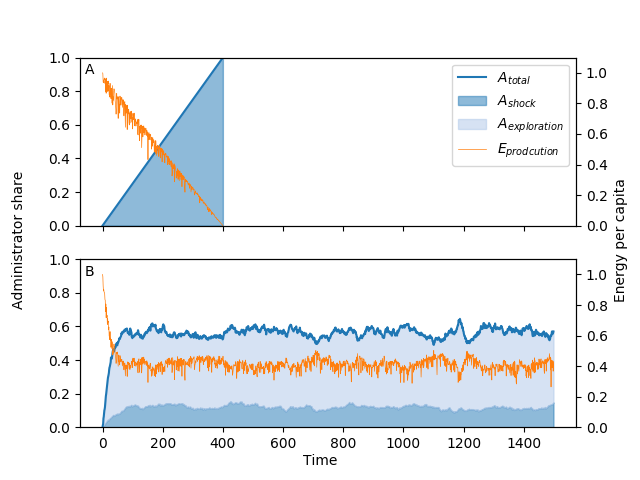
\includegraphics[width=\linewidth]{../figures/Admin_Ecap_twocases.png}
    \caption{Example of development of a society without capacity of exploration (i.e. random change from work to adminstration and vice versa). }
    \label{fig:baseNetworkDev}
\end{figure}


\paragraph{Interplay between network characteristics. Conditions for a beneficial administration}

Find out realistic ranges of efficiency and link density in simplistic societies, in order to be able to discuss the graphic




\begin{figure}[htb]
    \centering
    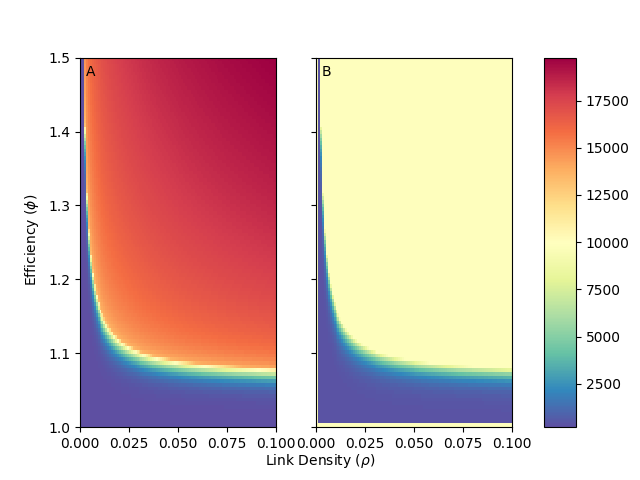
\includegraphics[width = \linewidth]{../figures/parscan_base0.png}
    \caption{Survival of a network with N = 400 as a function of exploration, link density and efficiency.}
    \label{fig:survival}
\end{figure}



\paragraph{Macroscopic approximation of original Tainter Dynamics}

\begin{figure}[htb]
    \centering
    \includegraphics[width = \linewidth]{../figures/comp_integration-model_exploration0.png}
    \caption{Survival of a network with N = 400 as a function of exploration, link density and efficiency.}
    \label{fig:survival}
\end{figure}

% P_e = 0 in order to leave out exploration term

\subsection{modified Tainter dynamics. Exploration}

\paragraph{model run description}

\paragraph{Low exploration results in highly increased survival times}

\paragraph{extension of macroscopic approximation}


% !TEX root = ../0_main/00_main.tex


% !TEX root = ../0_main/00_main.tex
\section{Conclusion}


\bibliographystyle{unsrt}
\bibliography{references}




\end{document}
